\documentclass[aspectratio=169]{beamer}

%\includeonlyframes{current}

\usepackage[utf8]{inputenc}
\usepackage[american]{babel}
\usepackage{amsmath,amsthm}
\usepackage{unicode}
\usepackage{array,tabularx}
\usepackage{ifthen}
\usepackage{tikz}
\usetikzlibrary{calc,arrows,arrows.meta,intersections}
\usepackage{tikzsymbols}

\usepackage{ulem}

\mode<presentation>{%
  \usetheme{ibm}
}

\newcommand{\C}{ℂ}
\newcommand{\R}{ℝ}
\newcommand{\Z}{ℤ}
\newcommand{\N}{ℕ}
\newcommand{\Q}{ℚ}
\newcommand{\F}{\mathbb{F}}
\renewcommand{\P}{\mathbb{P}}
\renewcommand{\O}{\mathcal{O}}
\newcommand{\tildO}{\mathcal{\tilde{O}}}
\newcommand{\poly}{\operatorname{poly}}
\newcommand{\polylog}{\operatorname{polylog}}
\newcommand{\End}{\operatorname{End}}
\newcommand{\Hom}{\operatorname{Hom}}
\newcommand{\Cl}{\operatorname{Cl}}
\newcommand{\GL}{\operatorname{GL}}
\newcommand{\SL}{\operatorname{SL}}
\newcommand{\cyc}[1]{{〈 #1 〉}}
\newcommand{\sm}[2]{\left(\protect\begin{smallmatrix}#1\protect\\#2\protect\end{smallmatrix}\right)}

\renewcommand{\a}{\mathfrak{a}}
\renewcommand{\b}{\mathfrak{b}}
\newcommand{\g}{\mathfrak{g}}
\newcommand{\G}{\mathcal{G}}
\newcommand{\E}{\mathcal{E}}
\DeclareMathOperator{\rank}{rank}

\title{The isogeny toolbox}
\author{Luca De Feo}
\date[October 1, 2024, Uni Torino]{October 1, 2024\\
  Seminario Algebra e Teoria dei Numeri, Università di Torino, Italy}
\institute{IBM Research Zürich}

\begin{document}

\frame[plain]{\titlepage}

%%

\begin{frame}{Diffie--Hellman key exchange}
  \begin{description}
  \item[Goal:] Alice and Bob have never met before. They are chatting
    over a public channel, and want to agree on a \emph{shared secret}
    to start a private conversation.
  \item[Setup:] They agree on a (large) cyclic group
    $G=\langle g\rangle$ of order $N$.
  \end{description}

  \begin{center}
    \begin{tikzpicture}
      \node at (0,0) {\bf Alice};
      \node at (7,0) {\bf Bob};
      \node at (0,-1) {pick random \alert{$a\in\Z/N\Z$}};
      \node at (0,-1.5) {compute $A=g^a$};
      \node at (7,-1) {pick random \alert{$b\in\Z/N\Z$}};
      \node at (7,-1.5) {compute $B=g^b$};
      \draw[->]
      (1,-2) to node[auto] {$A$} (6,-2);
      \draw[->] (6,-2.5) to node[auto] {$B$} (1,-2.5);
      \node at (3.5,-3.5) {\emph{Shared secret} is \alert{$B^a=g^{ab}=A^b$}};
    \end{tikzpicture}
  \end{center}
\end{frame}

%%

\begin{frame}{Let~~~~$E \;:\; y^2 = x^3 + ax + b$~~~~be an elliptic curve\dots}

  \begin{center}
    \begin{tikzpicture}[domain=-2.4566:4,samples=100]
      \newcount\rotate
      \animate<2-6>
      \animatevalue<2-6>{\rotate}{0}{90}
      \begin{scope}[rotate=-\the\rotate]
        \draw plot (\x,{0.5*sqrt(\x*\x*\x-4*\x+5)});
        \draw plot (\x,{-0.5*sqrt(\x*\x*\x-4*\x+5)});
      \end{scope}
      
      \begin{uncoverenv}<1>
        \begin{scope}[yscale=1/2]
          \draw[thin,gray,-latex] (0,-7) -- (0,7);
          \draw[thin,gray,-latex] (-3,0) -- (4,0);
          
          \draw (-3,1) -- (4,8/3+3);
          \begin{scope}[every node/.style={draw,circle,inner sep=1pt,fill},cm={1,2/3,0,0,(0,3)}]
            \node at (-2.287980,0) {};
            \node at (-0.535051,0) {};
            \node at (3.267475,0) {};
          \end{scope}
          \begin{scope}[every node/.style={yshift=0.3cm},cm={1,2/3,0,0,(0,3)}]
            \node at (-2.287980,0) {$P$};
            \node at (-0.535051,0) {$Q$};
            \node at (3.267475,0) {$R$};
          \end{scope}
          \draw[dashed] (3.267475,3.267475*2/3+3) -- (3.267475,-3.267475*2/3-3) 
          node[draw,circle,inner sep=1pt,fill] {}
          node[xshift=-0.1cm,anchor=east] {$P+Q$};
        \end{scope}
      \end{uncoverenv}
    \end{tikzpicture}
  \end{center}
\end{frame}

%%

\begin{frame}{Let~~~~$E \;:\; y^2 = x^3 + ax + b$~~~~be an elliptic curve\dots}
  \transdissolve
  \centering
  \includegraphics[height=0.7\textheight]{ec-happy}
\end{frame}

%%

\begin{frame}{The Quantum Menace}
  \centering
  \includegraphics[height=0.7\textheight]{qc-color}
\end{frame}

%% 

\begin{frame}{Post-quantum Cryptography \small(digital signatures overview, September 2024)}
  \centering
  \includegraphics[height=0.9\textheight]{onramp-rnd1.pdf}
\end{frame}

%%

\begin{frame}{From Elliptic Curve to Isogeny-based Cryptography}
  \Large
  \begin{description}
    \setlength{\itemsep}{4em}
  \item[Isogenies =] finite-kernel \textit{algebraic} group morphisms: \emph{$E \to E'$}
  \item[Endomorphisms =] isogenies \emph{$E \to E$}
  \end{description}
\end{frame}

%%

\begin{frame}{Isogenies: an example over $\F_{11}$}
  \centering
  \begin{tikzpicture}[scale=0.4]
    \begin{scope}
      \node[anchor=center] at (0,7) {$E \;:\; y^2 = x^3 + x$};

      \uncover<-1>{
        \draw[thin,gray] (0,-6) -- (0,6);
        \draw[thin,gray] (-6,0) -- (6,0);
      }

      \foreach \x/\y in {0/0,5/3,-4/3,-3/5,-2/1,-1/3} {
        \draw[blue,fill] (\x,\y) circle (0.2) node(E_\x_\y){}
        (\x,-\y) circle (0.2) node(E_\x_-\y){};
      }

      \uncover<2->{\draw[red,fill] (0,0) circle (0.3);}
    \end{scope}

    \draw[black!10!white,thick] (10,-7) -- +(0,14);
    
    \begin{scope}[shift={(20,0)}]
      \node at (0,7) {$E' \;:\; y^2 = x^3 - 4x$};

      \uncover<-1>{
        \draw[thin,gray] (0,-6) -- (0,6);
        \draw[thin,gray] (-6,0) -- (6,0);
      }

      \foreach \x/\y in {0/0,2/0,3/2,4/2,6/4,-2/0,-1/5} {
        \draw[color=blue,fill] (\x,\y) circle (0.2) node(F_\x_\y){}
        (\x,-\y) circle (0.2) node(F_\x_-\y){};
      }
    \end{scope}

    \begin{scope}[color=red,-latex,dashed]
      \begin{uncoverenv}<2->
        \path
        (E_5_3) edge (F_3_2)
        (E_-4_3) edge (F_4_-2)
        (E_-3_5) edge (F_4_2)
        (E_-2_1) edge (F_3_-2)
        (E_-1_3) edge (F_-2_0);
      \end{uncoverenv}
      \begin{uncoverenv}<2->
        \path
        (E_5_-3) edge (F_3_-2)
        (E_-4_-3) edge (F_4_2)
        (E_-3_-5) edge (F_4_-2)
        (E_-2_-1) edge (F_3_2)
        (E_-1_-3) edge (F_-2_0);
      \end{uncoverenv}
    \end{scope}
  \end{tikzpicture}
  
  \begin{columns}
    \begin{column}{0.5\textwidth}
      \[\phi(x,y) = \left(\frac{x^2 + 1}{x},\quad y\frac{x^2-1}{x^2}\right)\]
    \end{column}
    \begin{column}{0.5\textwidth}
      \begin{itemize}
      \item<2-> Kernel generator in \alert{red}.
      \item<2-> This is a degree $2$ map.
      \item<2-> Analogous to $x\mapsto x^2$ in $\F_q^*$.
      \end{itemize}
    \end{column}
  \end{columns}
\end{frame}

%%

\begin{frame}{Degree and dual}
  \large
  Let \emph{$φ : E \to E'$}. There exist:

  \smallskip
  \begin{uncoverenv}<2->
    \begin{description}
    \item[Degree:] a smallest integer \emph{$d > 0$}, and
    \item[Dual:] a unique isogeny \emph{$\widehat{φ} : E' \to E$},
    \item<3-> such that:
    \end{description}
  \end{uncoverenv}
  
  \medskip
  \centering
  \begin{tikzpicture}
    \node (E1) at (6,0) {$E'$};
    \node (E) at (0,0) {$E$};

    \draw[-latex] (E) edge[bend left] node[above] {$φ$} (E1);

    \uncover<2->{
      \draw[-latex] (E1) edge[bend left] node[below] {$\widehat{φ}$} (E);
    }
    
    \uncover<3->{
      \draw[-latex] (E1) edge[loop,out=45,in=-45,looseness=10] node[right] {mul.\ by $d$} (E1);
      \draw[-latex] (E) edge[loop,out=135,in=225,looseness=10] node[left] {mul.\ by $d$} (E);
    }
  \end{tikzpicture}
\end{frame}

%%

\begin{frame}{Anatomy of an isogeny}
  \transdissolve<2-8>
  \large
  \centering
  \begin{tikzpicture}
    \node at (-6,0) {$\phi(x,y) = \Biggl($};
    \node (x) at (-2.5,0) {$\displaystyle
      \frac{
        \only<-6>{x^4 - x^3 + 11x^2 + 9x + 12}
        \only<7->{g(x)}
      }{
        \only<-3>{\phantom{(}x^3-x^2-x+1\phantom{)}}
        \only<4-5>{(x + 1)(x - 1)^2}
        \only<6->{h(x)}
      },$};
    \node (y) at (3.5,0) {$\displaystyle y
      \only<-7>{\frac{x^5 - x^4 - 14x^3 - 26x^2 - 67x - 21}{x^5 - x^4 - 2x^3 + 2x^2 + x - 1}}
      \only<8->{\left(\frac{g(x)}{h(x)}\right)'}$};
    \node at (7,0) {$\Biggr)$};
    
    \begin{scope}[thick,red]
      \uncover<2-6>{\draw (-4.5,0.4) circle (0.2) +(0,0.2) -- +(0,1) +(0,1.2) node {degree};}
      \uncover<2>{\draw (-3.6,-0.2) circle (0.2) +(0,-0.2) -- +(0,-1) +(0,-1.2) node {degree $-1$};}
      \uncover<3-4>{
        \draw (-2.5,-0.3) ellipse (1.7 and 0.4) +(0,-0.4) -- +(0,-1.2) +(0,-1.4) node {kernel polynomial};
      }
      \uncover<5>{
        \draw (-3.3,-0.3) ellipse (0.7 and 0.4) +(-0.5,-0.3) -- +(-1,-0.6) +(-1.2,-0.8) node {Point of order $2$};
        \draw (-1.9,-0.3) ellipse (0.9 and 0.4) +(0.2,-0.4) -- +(1,-1.5) +(1.1,-1.7) node {Two points of order $4$};
      }
      \uncover<6->{
        \draw (-2.5,-0.6) -- +(0,-1) +(0,-1.5) node {$h(x) = \displaystyle\prod_{P\in K\setminus\{0\}}\bigl(x-x(P)\bigr)$};
      }
      \uncover<7->{
        \draw (-2.5,0.6) -- +(0,1) +(0,1.5) node {computed by Vélu--Elkies--Kohel formulas};
      }
    \end{scope}
  \end{tikzpicture}

  \medskip
  
  \begin{uncoverenv}<9->
    \begin{description}
    \item[Input:] Finite kernel \emph{$K⊂E$} of order \emph{$d$};
    \item[Output:] Rational fractions \emph{$ϕ(x,y)$};
    \item[Complexity:] \emph{$\tilde{O}(d)$} operations.
    \end{description}
  \end{uncoverenv}
\end{frame}

%%

\begin{frame}{How many isogenies?}
  \large
  \begin{tikzpicture}
    \node (K) at (-4, 0) {
      \begin{minipage}{6cm}
        \centering
        Finite subgroups of order $d$
        \[\emph{K ⊂ E}\]
      \end{minipage}
    };
    \node (I) at (4, 0) {
      \begin{minipage}{6cm}
        \centering
        Isogenies of degree $d$
        \[\emph{\phi: E \to E/K}\]
        {\normalsize (up to composing with isomorphism)}
      \end{minipage}
    };
    \draw[latex-latex] (K) edge (I);
  \end{tikzpicture}

  \pause
  \vfill

  \emph{Examples:}

  \begin{table}
    \begin{tabular}{l l}
      If $d$ is prime &$→$ at most \emph{$d+1$} possible kernels,\\[0.5em]
      In general      &$→$ at most \emph{$≈ d$} possible kernels.
    \end{tabular}
  \end{table}
\end{frame}

%%

\begin{frame}{The isogeny problem}
  \Large\centering
  \begin{tikzpicture}[scale=2]
    \node (E) at (0,0) {$E$};
    \node (E1) at (4,0) {$E'$};
    \uncover<2->{
      \draw[-latex] (E) edge node[above] {??} (E1);
    }
  \end{tikzpicture}
\end{frame}

%%

\begin{frame}{Isogeny graphs}
  \large
  \begin{columns}
    \begin{column}{0.45\textwidth}
      \[
        \frac{x^2 + \cdots}{x + \cdots}
        \uncover<2->{\circ\frac{x^2 + \cdots}{x + \cdots}}
        \uncover<3->{\circ\frac{x^2 + \cdots}{x + \cdots}}
        \uncover<4->{\circ\frac{x^2 + \cdots}{x + \cdots}}
      \]
    \end{column}
    \begin{column}{0.55\textwidth}
      \centering
      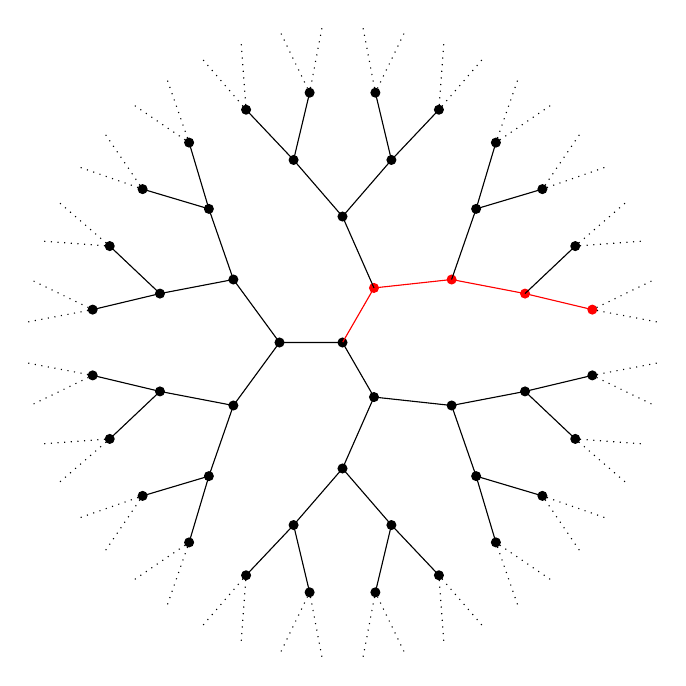
\begin{tikzpicture}[scale=0.8]
        \def\levels{5}
        \draw[fill] (0:0) circle (2pt);
        \foreach \i in {1,...,\levels} {
          \pgfmathparse{3*2^\i}
          \let\nodes\pgfmathresult
          \foreach \j in {1,3,...,\nodes} {
            \pgfmathparse{\j + (-1)^div(\j,2)}
            \let\lower\pgfmathresult
            \uncover<\i->{
              \ifthenelse{\i = \levels}{
                \draw[dotted] (360/\nodes*\j : \i) --
                (360/\nodes*\lower : \i - 1);
              }{
                \pgfextra{
                  \ifthenelse{\j=1}{\def\col{red}}{\def\col{black}}
                  \draw[fill,\col] (360/\nodes*\j : \i) circle (2pt) --
                  (360/\nodes*\lower : \i - 1);
                }
              }
            }
          }
        }
      \end{tikzpicture}
    \end{column}
  \end{columns}
\end{frame}

%%

\begin{frame}{Legend}
  \large
  \begin{tikzpicture}[anchor=west]
    \draw[very thick] (0,0) edge[-{>[scale=2]}] +(2,0) 
    ++(4,0) node{\emph{smooth} decomposition}
    ++(5,0) node{$φ = φ_n∘\cdots∘φ_1$};
  \end{tikzpicture}
\end{frame}

%%

\begin{frame}{The \textit{smooth} criminals}
  \Large
  \begin{columns}
    \begin{column}{0.7\textwidth}
      \begin{description}
        \setlength{\itemsep}{1em}
      \item[2006] Charles-Goren-Lauter hash function
      \item[2006] Couveignes-Rostovtsev-Stolbunov key exchange
      \item[2011] SIDH key exchange~~~\emph{($\dagger$ 2022)}\\ {\small(Jao, D.)}
      \item[2018] CSIDH key exchange\\ {\small(Castryck, Lange, Martindale,
        Panny, Renes)}
      \end{description}
    \end{column}
    \begin{column}{0.3\textwidth}
      \includegraphics[height=0.8\textheight]{smooth-criminal}
    \end{column}
  \end{columns}
\end{frame}

%%

\begin{frame}{Lattices of isogenies}
  \centering
  \begin{tikzpicture}
    \large
    \node (E1) at (0,0) {$E'$};
    \node (E) at (6,0) {$E$};
    \uncover<2->{
      \draw[dashed,->] (E) edge node[above]
      {$\uncover<3->{\alert{a}}φ+\uncover<3->{\alert{b}}ψ$} (E1);
    }
    
    \draw[->] (E) edge[bend right] node[above] {$φ$} (E1)
    edge[bend left] node[above] {$ψ$} (E1);
    \node at (9,1) {$φ,ψ ∈ \Hom(E,E')$};
    \uncover<3->{
      \node at (12,1) {\alert{$a,b∈ℤ$}};
    }

    \uncover<2->{
      \node at (10,-1) {$(\uncover<3->{\alert{a}}φ + \uncover<3->{\alert{b}}ψ)(P)
        :=
        \uncover<3->{[\alert{a}]}φ(P) + \uncover<3->{[\alert{b}]}ψ(P)$};
    }
  \end{tikzpicture}

  \bigskip
  
  \uncover<4->{
    \begin{itemize}
      \setlength{\itemsep}{1.5em}
    \item $\deg(aφ) = a^2\deg(φ)$,
    \item $\big\lvert \deg(φ+ψ) - \deg(φ) - \deg(ψ) \big\rvert ≤ 2\sqrt{\deg(φ)\deg(ψ)}$,
    \item $\deg$ is a \emph{positive definite quadratic form.}
    \end{itemize}
  }
\end{frame}

%%

\begin{frame}{Endomorphism rings}
  \large
  \begin{itemize}
    \setlength{\itemsep}{2em}
  \item $\Hom(A,B)$: additive group
  \item Distributivity:
    \begin{align*}
      φ∘(ψ+χ) &= (φ∘ψ)+(φ∘χ)\\[2em]
      (ψ+χ)∘φ &= (ψ∘φ)+(χ∘φ)\\
    \end{align*}
  \item It follows that \emph{$\End(A) := \Hom(A,A)$} is a ring.
  \end{itemize}  
\end{frame}

%%

\begin{frame}{Endomorphism rings}
  \large $\End(E)$ is a free $ℤ$-module of rank \textcolor{blue}{1},
  \textcolor{purple}{2} or \textcolor{red}{4}. As a ring:

  \bigskip
  \begin{enumerate}
    \setlength{\itemsep}{1em}
  \item[\color{blue}1)] $\End(E) ≃ ℤ$;
  \item[\color{purple}2)] $\End(E) ⊂$ quadratic imaginary field;
  \item[\color{red}4)] $\End(E) ⊂$ quaternion algebra.
  \end{enumerate}
\end{frame}

%%

\begin{frame}{Isogenies = $\End(E)$-Ideals}
  \large\centering
  \begin{tikzpicture}
    \node (E1) at (0,0) {$E'$};
    \node (E) at (6,0) {$E$};

    \draw[-latex] (E) edge node[above] {$φ$} (E1);
    \uncover<1>{
      \node at (3,-3) {$φ ∈ \Hom(E,E')$};
    }

    \uncover<2>{
      \draw[-latex] (E) edge[loop,out=45,in=-45,looseness=10] node[right] {$ω$} (E);
      \node at (3,-3) {$φ∘ω ∈ \Hom(E,E')$};
    }
    
    \uncover<3>{
      \draw[-latex] (E1) edge[loop,out=135,in=225,looseness=10] node[left] {$ω'$} (E1);
      \node at (3,-3) {$ω'∘φ ∈ \Hom(E,E')$};
    }
  \end{tikzpicture}
\end{frame}

%%

\begin{frame}{The Deuring correspondence: Isogenies $\longleftrightarrow$ Ideals}
  \large $\Hom(E,E')$ is a free $ℤ$-module of rank
  \textcolor{blue}{1}, \textcolor{purple}{2} or \textcolor{red}{4}.

  \bigskip
  It is a \emph{rank-1} projective $\End(E)$-module, isomorphic to:

  \bigskip
  \begin{enumerate}
    \setlength{\itemsep}{1em}
  \item[\color{blue}1)] an ideal of \textcolor{blue}{$ℤ$};
  \item[\color{purple}2)] an invertible ideal of a
    \textcolor{purple}{quadratic imaginary field};
  \item[\color{red}4)] an invertible ideal of a
    \textcolor{red}{quaternion algebra}.
  \end{enumerate}

  \bigskip
  As a quadratic module: \emph{degree $\longleftrightarrow$ norm}
\end{frame}

%%

\begin{frame}{The Deuring correspondence: Isogenies $\longleftrightarrow$ Ideal classes}
  \Large
  \begin{description}
    \setlength{\itemsep}{2em}
  \item[Equivalent ideals:]
    \[I ≃ J  \quad\Longleftrightarrow\quad I = Jα\]
  \item[Deuring correspondence:]
    \[\Hom(E,E') \quad\longleftrightarrow\quad \mathrm{cls}(I)\]
  \end{description}
\end{frame}

%% 

\begin{frame}{Two computational worlds}
  \centering
  \setlength{\tabcolsep}{2em}
  \renewcommand{\arraystretch}{1.5}
  \begin{tabular}{p{0.3\textwidth} c c}
    & \textcolor{purple}{Quadratic imaginary} & \textcolor{red}{Quaternionic}\\
    \hline
    $\rank\Hom(E,E')$ & 2 & 4\\
    Endomorphism algebra & number field & quaternion algebra\\
    Maximal orders & one & many \\
    Ideal class\dots & \dots group & \dots set\\
    Find isogeny $E → E'$ & \alert{hard} & \alert{hard}\\
    Convert isogenies $\leftrightarrow$ ideals & easy-ish\footnotemark[1] & easy\footnote[1]{When $\End(E)$ is known}\\
    Compute $\End(E)$ & easy & \alert{hard}\\
  \end{tabular}
\end{frame}

%%

\begin{frame}{The quadratic imaginary case}
  \begin{block}{Complex Multiplication}
    Fix an order \emph{$\O ⊂ ℚ(\sqrt{-D})$}:
    \begin{itemize}
    \item Invertible ideal classes form a \emph{finite abelian group}
    \item $\Cl(\O)$ acts \emph{freely and transitively} on the set of
      elliptic curves with $\End(E) ≃ \O$.
    \end{itemize}
  \end{block}
\end{frame}

%%

\begin{frame}{Key exchange from group actions}
  \begin{description}
  \item[Public parameters:]
    \begin{minipage}{0.6\linewidth}
      \begin{itemize}
      \item A starting elliptic curve $E_0$;
      \item $\End(E) ≃ \O ⊂ ℚ(\sqrt{-D})$.
      \end{itemize}
    \end{minipage}
  \end{description}

  \bigskip
  
  \begin{center}
    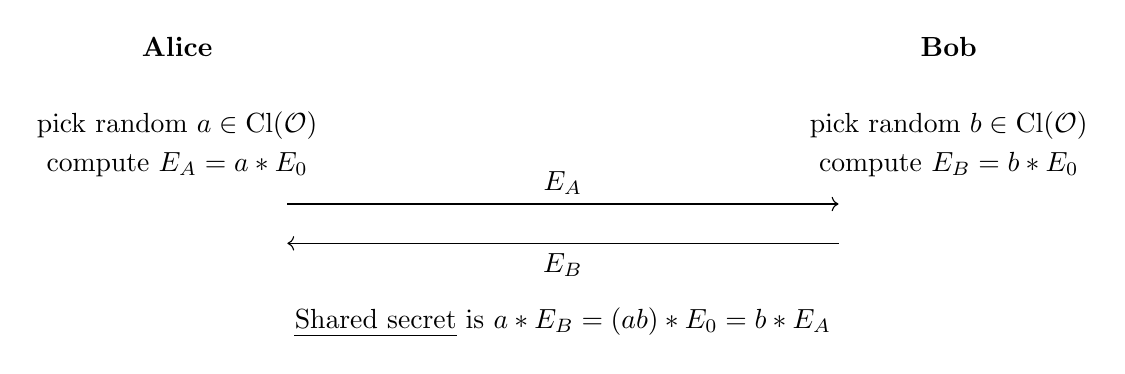
\begin{tikzpicture}[x=1.4cm]
      \node at (0,0) {\bf Alice};
      \node at (7,0) {\bf Bob};
      \node at (0,-1) {pick random \alert{$\a\in\Cl(\O)$}};
      \node at (0,-1.5) {compute $E_A=\a*E_0$};
      \node at (7,-1) {pick random \alert{$\b\in\Cl(\O)$}};
      \node at (7,-1.5) {compute $E_B=\b*E_0$};
      \draw[->]
      (1,-2) to node[auto] {$E_A$} (6,-2);
      \draw[->] (6,-2.5) to node[auto] {$E_B$} (1,-2.5);
      \node at (3.5,-3.5) {\emph{Shared secret} is \alert{$\a*E_B=(\a\b)*E_0=\b*E_A$}};
    \end{tikzpicture}
  \end{center}
\end{frame}

%%

\begin{frame}{Two computational worlds}
  \centering
  \setlength{\tabcolsep}{2em}
  \renewcommand{\arraystretch}{1.5}
  \begin{tabular}{p{0.3\textwidth} c c}
    & \textcolor{purple}{Quadratic imaginary} & \textcolor{red}{Quaternionic}\\
    \hline
    $\rank\Hom(E,E')$ & 2 & 4\\
    Endomorphism algebra & number field & quaternion algebra\\
    Maximal orders & one & many \\
    Ideal class\dots & \dots group & \dots set\\
    Find isogeny $E → E'$ & \alert{hard} & \alert{hard}\\
    Convert isogenies $\leftrightarrow$ ideals & easy-ish\footnotemark[1] & easy\footnote[1]{When $\End(E)$ is known}\\
    Compute $\End(E)$ & easy & \alert{hard}\\
  \end{tabular}
\end{frame}

%%

\begin{frame}{The endomorphism ring problem}
  \Large\centering
  \vfill
  Given a random supersingular curve $E$, compute $\End(E)$
  \vfill
\end{frame}

%%

\begin{frame}{Contagious knowledge}
  \centering
  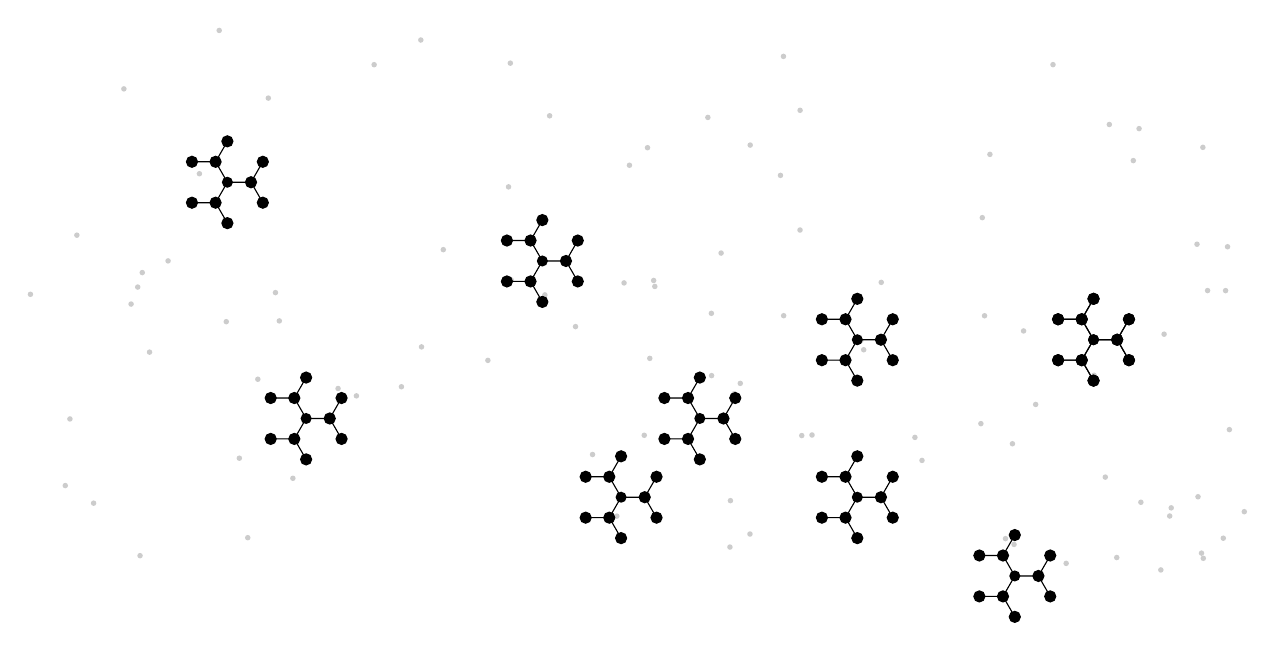
\begin{tikzpicture}
    \pgfmathsetseed{12345}
    \foreach \i in {1,...,100} {
      \pgfmathparse{16*random()}
      \let\x\pgfmathresult
      \pgfmathparse{7*random()}
      \let\y\pgfmathresult
      \fill[black!20!white] (\x,\y) circle (1pt);
    }
    \foreach \i in {1,...,10} {
      \pgfmathparse{floor(15*random())}
      \let\x\pgfmathresult
      \pgfmathparse{floor(6*random())}
      \let\y\pgfmathresult
      \fill (\x,\y) circle (2pt);
      \uncover<2->{
        \foreach \rho in {0,1,2} {
          \draw[fill,-latex] (\x,\y) -- +(120*\rho:.3) circle (2pt);
          \uncover<3->{
            \foreach \sigma in {-1,1} {
              \draw[fill,-latex] (\x,\y) ++(120*\rho:.3) -- ++(120*\rho+60*\sigma:.3) circle (2pt);
            }
          }
        }
      }
    }
  \end{tikzpicture}
\end{frame}

%%

\begin{frame}{Legend}
  \large
  \begin{tikzpicture}[anchor=west]
    \draw[very thick] (0,0) edge[-{>[scale=2]}] +(2,0) 
    ++(4,0) node{\emph{smooth} decomposition}
    ++(5,0) node{$φ = φ_n∘\cdots∘φ_1$};
    %%
    \draw[very thick] (0,-2) edge[-{[scale=2]>>>>}] +(2,0) 
    ++(4,0) node{Deuring representation}
    ++(5,0) node{$α = aφ + bψ + cχ + dω$};
    
  \end{tikzpicture}
\end{frame}

%%

\begin{frame}{Deuring representation in action}
  \Large
  \begin{description}
    \setlength{\itemsep}{1em}
  \item[2016] Galbraith-Petit-Silva signature scheme
  \item[2019] CSI-FiSh signature scheme\\
    {\small (Beullens, Kleinjung, Vercauteren)}
  \item[2020] SQIsign signature scheme\\
    {\small (D., Kohel, Leroux, Petit, Wesolowski)}
  \end{description}
\end{frame}

%%

\begin{frame}{SQIsign \small(identification scheme)}
  \transdissolve<4,6>
  \large
  \centering
  \begin{tikzpicture}[very thick]
    \fill
    (0,3) node(E0){} circle (4pt);
    \draw
    (-4,0) node(PK){} circle (4pt);
    \draw[dashed,->>>>] (PK) edge node[above,sloped] {secret key} (E0);
    
    \uncover<2->{
      \draw (6,3) node(COM){} circle (4pt);
      \draw[dashed,->>>>] (E0) edge node[sloped,above] {commitment} (COM);
    }

    \uncover<3->{
      \draw (10,0) node(CH){} circle (4pt);
    }
    \uncover<3,6->{
      \draw (COM) edge[->] node[sloped,above] {challenge} (CH);
    }

    \uncover<4-5>{
      \draw (COM) edge[dashed,->>>>] node[sloped,above] {challenge} (CH);
    }

    \uncover<5>{
      \draw (PK) edge[dashed,->>>>] (CH);
    }

    \uncover<6->{
      \node at (3,1.5) {\includegraphics[height=2cm]{wizard-hat}};
      \node at (3.7,0.8) {\small KLPT};
      \draw (PK) edge[->] node[below] {response} (CH);
    }
  \end{tikzpicture}
\end{frame}

%%

\begin{frame}{Higher dimensional abelian varieties}
  \centering
  \begin{tikzpicture}[domain=-2.4566:4,samples=100]
    \begin{scope}[xscale=0.3,yscale=0.5]
      \draw plot (\x,{sqrt(\x*\x*\x-4*\x+5)});
      \draw plot (\x,{-sqrt(\x*\x*\x-4*\x+5)});
      \node (P1) at (3,4.47213595499958) {};
    \end{scope}
    \begin{uncoverenv}<2->
      \begin{scope}[xscale=0.7,yscale=0.15,shift={(7,-20)}]
        \draw plot ({sqrt(\x*\x*\x-4*\x+5)},\x);
        \draw plot ({-sqrt(\x*\x*\x-4*\x+5)},\x);
        \node (P2) at (-4.47213595499958,3) {};
      \end{scope}
      \node at (5,0) {\huge $E×E$};
      
      \fill (P1) circle (2pt);
      \fill (P2) circle (2pt);

      \draw[dashed] (P2) -- (P2 |-, |- P1) -- (P1);
      \fill (P2 |-, |- P1) circle (2pt) node[above right] {$(P,Q)$};
    \end{uncoverenv}
  \end{tikzpicture}
\end{frame}

%%

\begin{frame}{Higher dimensional isogenies}
  \large
  \begin{columns}
    \begin{column}{0.4\textwidth}
      \centering
      \begin{tikzpicture}[scale=2]
        \uncover<2->{
          \node (A) at (-1,1) {$A$};
          \node (B) at (1,-1) {$B$};
          \node (C) at (1,1) {$C$};
          \node (D) at (-1,-1) {$D$};
          
          \draw[-latex] (A) edge node[above] {$α$} (C) edge node[left] {$β$} (D)
          (B) edge node[right] {$γ$} (C) edge node[below] {$δ$} (D);
        }
      \end{tikzpicture}
    \end{column}
    \begin{column}{0.6\textwidth}
      \begin{align*}
        A × B &→ C × D\\
        \uncover<2->{(P,Q) &↦ \bigl( α(P) + γ(Q), β(P) + δ(Q) \bigr)}\\
              &\uncover<3->{=
                \begin{pmatrix}
                  α&γ\\β&δ
                \end{pmatrix}
                \begin{pmatrix}
                  P\\Q
                \end{pmatrix}}
      \end{align*}
    \end{column}
  \end{columns}
\end{frame}

%%

\begin{frame}{Higher dimensional embeddings (Kani's lemma)}
  \large
  \begin{columns}
    \begin{column}{0.4\textwidth}
      \centering
      \begin{tikzpicture}[scale=2]
        \node (A) at (-1,1) {$A$};
        \node (C) at (1,1) {$C$};
        
        \draw[-latex] (A) edge node[above] {$α$} (C);
        
        \uncover<2->{
          \node (B) at (1,-1) {$B$};
          \node (D) at (-1,-1) {$D$};

          \node at (0,0) {\Huge $\circlearrowleft$};

          \draw[-latex]
          (A) edge node[left] {$β$} (D)
          (B) edge node[right] {$\overline{β}$} (C)
          edge node[below] {$\overline{α}$} (D);
        }
      \end{tikzpicture}
    \end{column}
    \begin{column}{0.6\textwidth}
      \uncover<3->{
        \begin{align*}
          Φ : A × B &→ C × D\\
          (P,Q) &↦ \bigl( α(P) + \overline{β}(Q), β(P) + \overline{α}(Q) \bigr)\\
                    &=\begin{pmatrix}
                      α&\overline{β}\\β&\overline{α}
                    \end{pmatrix}
                      \begin{pmatrix}
                        P\\Q
                      \end{pmatrix}
        \end{align*}
      }

      \begin{enumerate}
      \item<4-> $Φ(P,0) = \bigl( \emph{α(P)}, -β(P) \bigr)$.
      \item<5-> $\deg Φ = \emph{\deg α + \deg β}$,
      \end{enumerate}
    \end{column}
  \end{columns}
\end{frame}

%%

\begin{frame}{Legend}
  \large
  \begin{tikzpicture}[anchor=west]
    \draw[very thick] (0,0) edge[-{>[scale=2]}] +(2,0) 
    ++(4,0) node{\emph{smooth} decomposition}
    ++(5,0) node{$φ = φ_n∘\cdots∘φ_1$};
    %%
    \draw[very thick] (0,-2) edge[-{[scale=2]>>>>}] +(2,0) 
    ++(4,0) node{\emph{Deuring} representation}
    ++(5,0) node{$α = aφ + bψ + cχ + dω$};
    %%
    \draw[very thick] (0,-4) edge[double distance=5pt,-Implies] +(2,0) 
    ++(4,0) node{\emph{HD} embedding}
    ++(5,0) node{$Φ(P,Q) =
      \left(\begin{smallmatrix}
        α&\overline{β}\\β&\overline{α}
      \end{smallmatrix}\right)
    \left(\begin{smallmatrix}
      P\\Q
    \end{smallmatrix}\right)$};
  \end{tikzpicture}
\end{frame}

%%

\begin{frame}{Gone HD}
  \Large
  \begin{description}
    \setlength{\itemsep}{1em}
  \item[2022] SIDH attacks\\
    {\small (Castryck, Decru ~/~ Maino, Martindale ~/~ Robert)}
  \item[2023]<2-> FESTA encryption scheme\\
    {\small (Basso, Maino, Pope)}
  \item[2023]<2-> SQIsignHD signature\\
    {\small (Dartois, Leroux, Robert, Wesolowski)}
  \item[2023]<2-> SCALLOP-HD key exchange\\
    {\small (Chen, Leroux, Panny)}
  \end{description}
\end{frame}

%%

\begin{frame}{Legend}
  \large
  \begin{tikzpicture}[anchor=west]
    \draw[very thick] (0,0) edge[-{>[scale=2]}] +(2,0) 
    ++(4,0) node{\emph{smooth} decomposition}
    ++(5,0) node{$φ = φ_n∘\cdots∘φ_1$};
    %%
    \draw[very thick] (0,-2) edge[-{[scale=2]>>>>}] +(2,0) 
    ++(4,0) node{\emph{Deuring} representation}
    ++(5,0) node{$α = aφ + bψ + cχ + dω$};
    %%
    \draw[very thick] (0,-4) edge[double distance=5pt,-Implies] +(2,0) 
    ++(4,0) node{\emph{HD} embedding}
    ++(5,0) node{$Φ(P,Q) =
      \left(\begin{smallmatrix}
        α&\overline{β}\\β&\overline{α}
      \end{smallmatrix}\right)
    \left(\begin{smallmatrix}
      P\\Q
    \end{smallmatrix}\right)$};
%%
\uncover<2->{
      \draw[very thick] (0,-6) edge[double distance=5pt,-{Implies[] Implies[] Implies[] Implies[]}] +(2,0) 
     ++(4,0) node{HD + Deuring = \emph{Clapoti} ~~\small(Page, Robert)};
}
\end{tikzpicture}
\end{frame}

%%

\begin{frame}{SQIsign2D}
  \transdissolve<4,6>
  \large
  \centering
  \begin{tikzpicture}[very thick]
    \fill
    (0,3) node(E0){} circle (4pt);
    \draw
    (4,3) node(PK){} circle (4pt);
    \draw (E0) edge[double distance=2pt,dashed,-{Implies[] Implies[] Implies[] Implies[]}] node[above,sloped] {secret key} (PK);
    
    \uncover<2->{
      \draw (-1,0) node(COM){} circle (4pt);
      \draw (COM) edge[double distance=2pt,dashed,-{Implies[] Implies[] Implies[] Implies[]}] node[sloped,above] {commitment} (E0);
    }

    \uncover<3->{
      \draw (5,0) node(CH){} circle (4pt);
    }
    \uncover<3,6->{
      \draw (PK) edge[->] node[sloped,above] {challenge} (CH);
    }

    \uncover<4-5>{
      \draw (PK) edge[double distance=2pt,dashed,-{Implies[] Implies[] Implies[] Implies[]}] node[sloped,above] {challenge} (CH);
    }

    \uncover<5>{
      \draw (COM) edge[double distance=2pt,dashed,-{Implies[] Implies[] Implies[] Implies[]}] (CH);
    }

    \uncover<6->{
      \node at (2,1.5) {\includegraphics[height=2cm]{wizard-hat}};
      \node at (2.7,0.8) {\small LLL};
      \draw (COM) edge[double distance=2pt,-Implies] node[below] {response} (CH);
    }
  \end{tikzpicture}
\end{frame}

%% 

\begin{frame}{SQIsign vs SQIsign2D}
  \large
  \begin{table}[h]
    \centering
    \begin{tabular}{ l r r | r r r | c }
      & Public Key & Signature & Keygen & Sign & Verify & Security \\
      \hline
      & 64 & 177 & 3,728 & 5,779 & 108 & NIST-1 \\
      SQIsign & 96 & 263 & 23,734 & 43,760 & 654 & NIST-3 \\
      & 128 & 335 & 91,049 & 158,544 & 2,177 & NIST-5 \\
      \hline
      \hline
      & 66 & 148 & 60 & 160 & 9 & NIST-1 \\
      SQIsign2D & 98 & 222 & 170 & 460 & 29 & NIST-3 \\
      & 130 & 294 & 360 & 940 & 62 & NIST-5 \\
      \hline
      & \multicolumn{2}{c|}{Bytes} & \multicolumn{3}{c|}{Mcycles}\\
    \end{tabular}
  \end{table}
\end{frame}

%%

\begin{frame}[plain]
  \centering
  \begin{tikzpicture}[remember picture,overlay]
    \begin{scope}[xscale=1.7,yshift=-15,opacity=0.8]
      \def\crater{12}
      \def\jumpa{-8}
      \def\jumpb{9}
      \def\diam{5cm}

      \foreach \i in {1,...,\crater} {
        \draw[blue] (360/\crater*\i : \diam) to[bend right] (360/\crater*\i+360/\crater : \diam);
        \draw[red] (360/\crater*\i : \diam) to[bend right] (360/\crater*\i+\jumpa*360/\crater : \diam);
        \draw[green] (360/\crater*\i : \diam) to[bend right=50] (360/\crater*\i+\jumpb*360/\crater : \diam);
      }
    \end{scope}
    
    
    \draw (0,0.5) node{\Huge\bf Thank you};
    \draw (0,-0.6) node{\large\url{https://defeo.lu/}};
    \draw (0,-1.3) node{\large\includegraphics[height=0.9em]{mastodon.png}~\href{https://twitter.com/luca_defeo}{@luca\_defeo@ioc.exchange}};
    \draw (0,-1.9) node{\large\includegraphics[height=0.9em]{twitter.png}~\href{https://twitter.com/luca_defeo}{@luca\_defeo}};
  \end{tikzpicture}
\end{frame}

\end{document}


% LocalWords:  Isogeny abelian isogenies hyperelliptic supersingular Frobenius
% LocalWords:  isogenous
